\Gls{ibc} systems as considered in this work are safety-critical. This requires a robustness study when such a system is subjected to approximations. To this end, we evaluate the failure probability of \gls{lkas} when subjected to different approximate settings (S1-S8). First, we perform Monte-Carlo simulations of the entire system while taking into account different approximate settings and environmental scenarios. Then, we obtain the percentage of lane misprediction and closed-loop failure probability of \gls{lkas}.

\subsection{Monte-Carlo simulation}
For Monte-Carlo simulation, we sweep different \gls{lkas} parameters in Webots using the \gls{hil} setup (Section~\ref{lkas_hil}) and obtain various system models for simulation. The considered parameters are initial starting position or initial lateral deviation of the vehicle, different weather conditions and different road surface types. From these simulations, the camera frames obtained by driving the vehicle are extracted and stored as a dataset for further analysis. For each frame in the dataset, the lane markings are annotated as \textit{ground truth} (information extracted from the accurate image). 

\subsection{Lane misprediction (LM)}\label{sec_lm}
Correct lane prediction is essential for proper \gls{lkas} operation. So, in this analysis, we study the sensitivity of the \gls{pr} stage to different approximate settings by calculating the increase in lane misprediction (LM) compared to the predictions using the \textit{ground truth}. 
We use the dataset obtained using Monte-Carlo simulations. Lane misprediction (LM) is calculated as shown below \cite{tusimple}:
\begin{equation} 
LM = 1 - \dfrac{1}{n}\sum_{i=1}^{n}\dfrac{PL_{i}}{G_{i}}
\nonumber
\end{equation}

where $PL_{i}$ is the number of correctly predicted lane points per frame and $G_{i}$ is the number of \textit{ground truth} points per frame. A prediction is considered correct if the difference between a \textit{ground truth} point and the predicted point is less than a certain threshold. $n$ is the total number of frames considered. In this work, $G_{i}$ = 512 and $n$ $=$ 3000. 
\begin{figure}[ht]
    \centering
    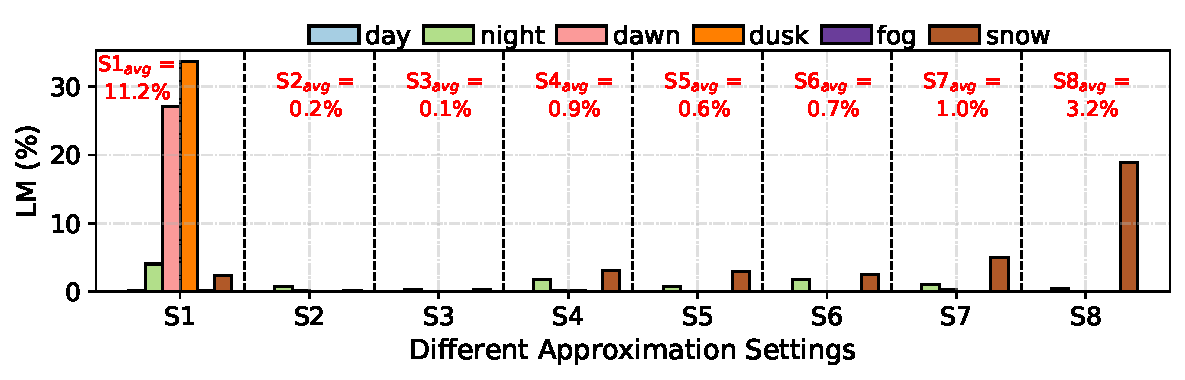
\includegraphics[width= \textwidth]{figs/lane_mispredict.pdf}
    \captionsetup{width=0.9\linewidth}
    \caption{{Sensitivity of \gls{pr} to different approximate settings when operating under different environmental scenarios. The average LM for each setting across all scenarios is shown in red.}}
    \label{fig:lm}
    % \vspace{-10 pt}
\end{figure}
Fig. \ref{fig:lm} shows that the \gls{pr} stage is robust to errors from approximation settings S2-S7 with average LM $\leq$ 1\%. We also see that image frames subjected to approximate settings S4-S7 have high visual changes (Fig. \ref{fig:qoc_wotime}) compared to the accurate one, but they still have low LM. This is because essential lane markings are not affected by these visual changes. Skipping denoising (S1) has a high negative impact on lane detection (PR) with average LM $=$ 11.7\%. Thus, skipping denoising (S1) while keeping the rest of the stages is not suitable for proper \gls{lkas} performance. We also observe that keeping only tone mapping (S8) works for all scenarios except snow (LM $=$ 18\%) which shows that scenario-based approximation selection is needed. 
  
\subsection{\Acrfull{fp}}
From the results of the previous subsection, we determine the worst-case approximation error (Section~\ref{lqg_control}) per setting considering the scenario with the highest LM for that setting. This error is used for designing different \gls{lqg} designs for \gls{fp} analysis.  We then calculate the failure probability of \gls{lkas} for different approximate settings (S1-S8) using Monte-Carlo simulations of the entire system. There are two questions that we need to address here: (a) Is the designed controller stable and robust? (b) Is there \gls{lkas} failure, i.e, does the vehicle go out of the lane?    
\par To evaluate stability robustness of the designed \gls{lqg} controller, we calculate the stability radius ($r$) which is the radius of the largest ball centered at the $(-1, 0)$ point to loop transfer function of the system in the nyquist plot \cite{lqg_robust}. $r$ is calculated as follows:
\begin{equation} 
r = \dfrac{1}{||S||_{\infty}}
\nonumber
\end{equation}

where $S$ is the sensitivity function calculated at the output of \gls{pr} for the proposed \gls{lkas} model and $0 \leq r \leq 1$. A higher value of $r$ means more stability robustness to sensor noise. The $r$ values obtained for S0-S8 are 0.8787, 0.9800, 0.9129, 0.9906, 0.9900, 0.9982, 0.9898, 0.9982 and 0.9999, respectively. All the $r$ values are close to 1, which shows the stability of the designed \gls{lqg} controllers. It is noted that the $r$ values for the approximate settings (S1-S8) are higher than the accurate (S0) one. This means that for the approximate cases, the \gls{lqg} contoller is designed to sustain a higher sensor noise margin. This has impact on the \gls{lqg} performance when evaluated in terms of \gls{fp}.
\par Failure probability of the \gls{lkas} is calculated as shown below:
\begin{equation} 
FP_{per\ km} = \dfrac{1}{m \times l}\sum_{i=1}^{m} F_{i}
\nonumber
\end{equation}

where $F_{i}$ is 1 if the number of times the vehicle goes out of the lane markings during the simulation interval is one or more; otherwise, it is 0. 
$m$ is the number of Monte-Carlo simulations performed for each approximate setting. For our experiments, we consider $m$ = 50000. $l$ is the lifetime of the vehicle. The typical lifetime of a conventional vehicle is 150,000~mi or 241,401.6~km~\cite{fault_tree}.

% \vspace{-10 pt}
\begin{figure}[ht]
    \centering
    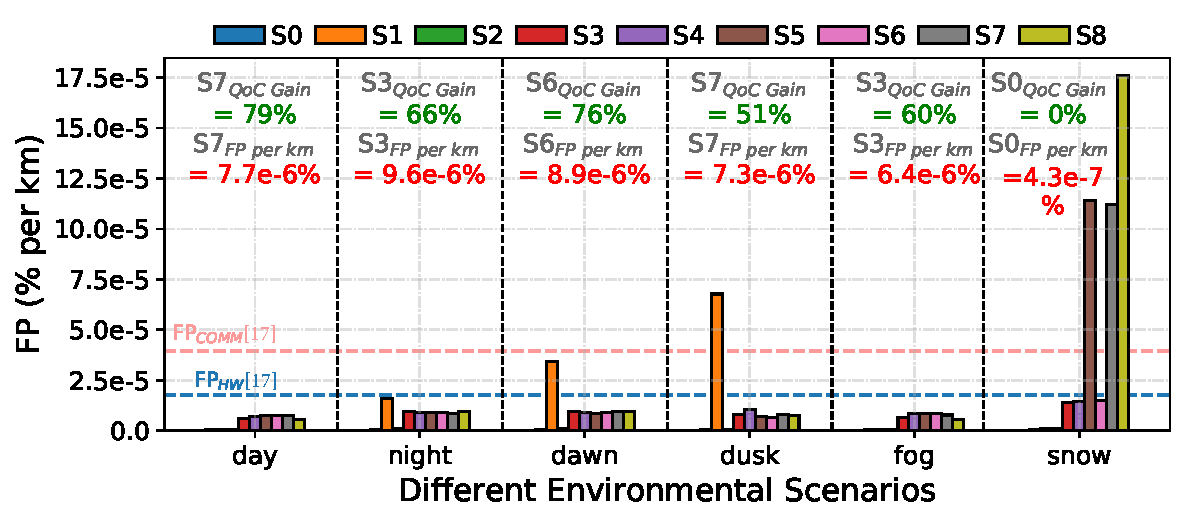
\includegraphics[width= 0.98\textwidth]{figs/fp.pdf}
    \captionsetup{width=0.9\linewidth}
    \caption{{Failure probability of \gls{lkas} for different approximate settings when operating under different environmental scenarios. Failure probability of the best performing setting per scenario is highlighted in red.}}
    \label{fig:fp}
    % \vspace{-5 pt}
\end{figure}

Fig.~\ref{fig:fp} shows the \gls{fp} of \gls{lkas} for different approximate settings under different environmental scenarios. To get some perspective, we plot the $FP_{per\ km}$ in the hardware and the communication subsystems of the vehicle as reported in \cite{fault_tree}. We notice that approximate settings S2, S3, S4 and S6 have a low failure probability across all scenarios. Considering the best performing (\gls{qoc}$_{best}$) setting per scenario, we notice that the system has worst-case $FP_{per\ km}$ of $9.6 \times 10^{-6}$\% (S3 for the night) which is well below the failure probabilities of the hardware and the communication subsystems \footnote{Software, hardware and communication subsystems are responsible for the majority of the autonomous vehicle failures related to vehicular components as reported in \cite{fault_tree}. Approximations proposed in this work contribute to software failure due to increased lane misprediction (LM). So, we report our results along with failure contributions due to discrepancies in hardware and communication subsystems to get a better perspective}.

% \vspace{-10 pt}
\begin{figure}[t]
    \centering
    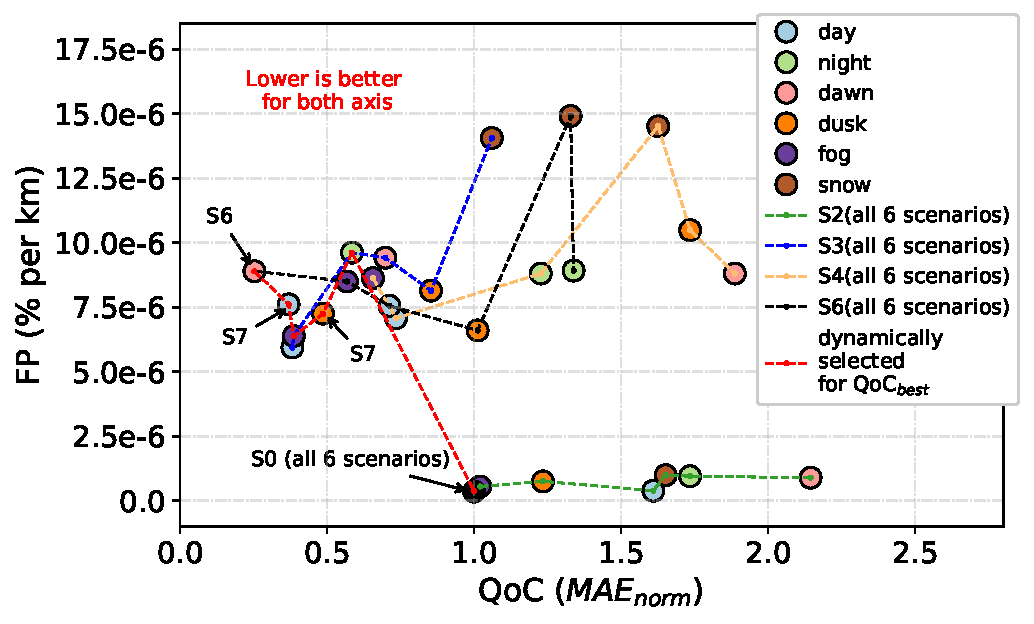
\includegraphics[width= 0.9\textwidth]{figs/fp_pareto_trim.pdf}
    %\vspace{-5pt}
    \captionsetup{width=0.9\linewidth}
    \caption{{Comparative study showing \gls{lkas} performance (\gls{qoc}) versus failure probability for the different approximate settings when operating under different environmental scenarios.}}
    \label{fig:fp_pareto}
    \vspace{-20 pt}
\end{figure}
Considering \gls{fp} in a standalone manner paints a partial picture. We are more interested in designs which not only have low \gls{fp} but also perform better than the accurate setting (S0). Fig. \ref{fig:fp_pareto} shows this comparative study between \gls{lkas} performance (\gls{qoc}) and $FP_{per\ km}$. \gls{qoc} values are normalized to the baseline (S0) for each scenario. S0 has the lowest \gls{fp} as expected. We start by comparing the four static approximate settings S2, S3, S4 and S6 which have low \gls{fp} across all scenarios. We observe that S2 has the lowest average \gls{fp} compared to S3, S4 and S6, but its closed-loop \gls{qoc} is worse than the baseline (S0) across all scenarios (see Fig.\ \ref{fig:fp_pareto}, green dotted line). Statically choosing S3, S4 and S6 across all scenarios shows improved \gls{qoc} compared to baseline for some scenarios and degraded \gls{qoc} for others (see Fig.\ \ref{fig:fp_pareto}, blue, yellow and black dotted lines). This motivates, as before, to dynamically select the approximate settings for each environmental scenario, which results in either improved or the same \gls{qoc} as that of the baseline (S0). This is shown by the red dotted line in Fig.\ \ref{fig:fp_pareto}. Note that we choose (from left to right on the red dotted line in Fig.\ \ref{fig:fp_pareto}) S6 for dawn, S7 for day, S3 for fog, S7 for dusk, S3 for night and S0 for the snow environmental scenarios for the best \gls{qoc}. A detailed analysis and the impact of switching between these scenarios at runtime is not in scope of this thesis. Interested readers are referred to \cite{de2021hardware}.   

The \gls{fp}, in the scope of this chapter on approximation, may be used as a cut-off criterion for choosing the acceptable (Pareto-optimal) approximate settings for different environmental scenarios at runtime. From Fig.\ \ref{fig:fp}, we can observe that most settings for different scenarios satisfy the cut-off criteria FP$_{COMM}$ and FP$_{HW}$ from the literature.
All the approximate settings that satisfy the \gls{fp} criteria can be deployed at runtime. The next criterion for choosing the Pareto-optimal approximate setting for a particular environment scenario is then the \gls{qoc}.
The outcomes after the \gls{fp} analysis from Fig.\ \ref{fig:fp_pareto} are the same as the results in Section \ref{robust} (as illustrated in Fig.\ \ref{fig:env_3}. This is as expected, given that the \gls{fp} shows that all the optimal settings found in Section \ref{robust} satisfy the \gls{fp} cut-off criterion. Note that in Fig.\ \ref{fig:fp_pareto}, the setting S3 has the lowest \gls{fp} for the day scenario, lower than setting S7. Since both S3 and S7 can be deployed at runtime due to low LM, we choose S7 that has a better \gls{qoc} compared to S3 for the day scenario.